\section{Input output}
Quando andiamo a parlare dei sistemi di input output le cose principale da considerare sono i 
disponsitivi di I/O i device controller, i buses, la gestione dell'I/O ed i device drivers.

\begin{figure}[!h]
    \centering
    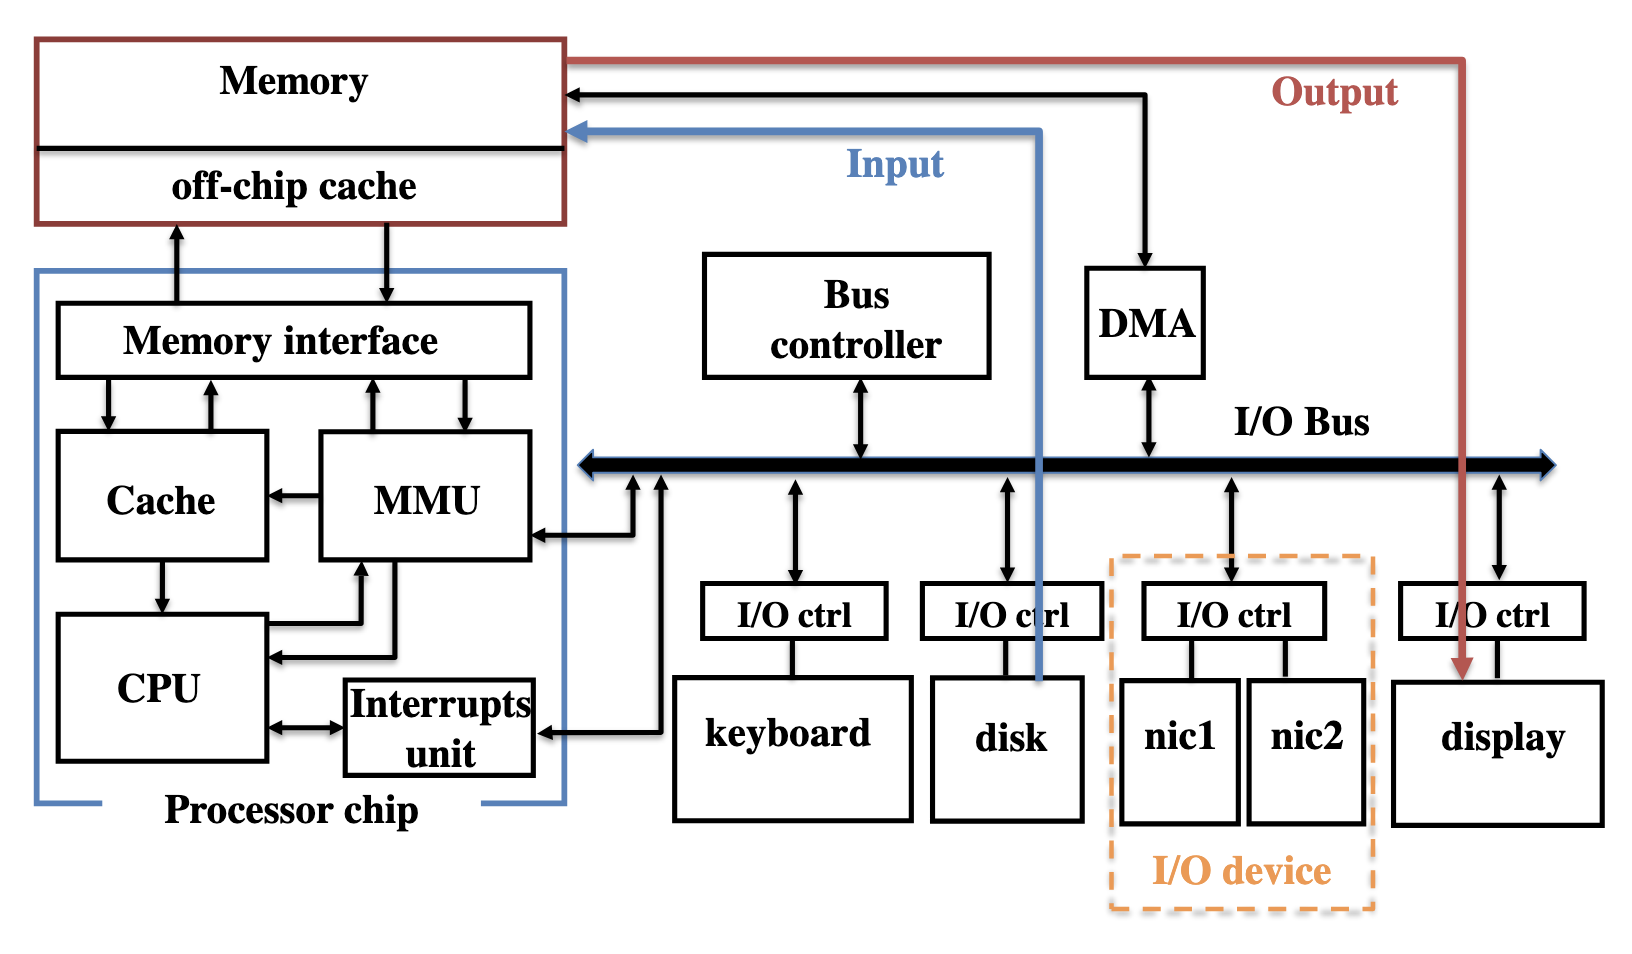
\includegraphics[width=13cm]{images/input-output-iodevice.png}
    \caption{Input/output e I/O devices}
\end{figure}

\hspace{-15pt}Solitamente le operazioni di I/O hanno un grosso impatto sul tempo di esecuzione dei programmi.
Supponiamo per esempio di andare a calcolare il tempo di esecuzione con \(T_{exe} = T_{cpu} + T_{I/O} = \frac{1}{10}T_{cpu}\) perciò
\(T_{exe} = \frac{11}{10}T_{cpu}\).\\\\
\hspace{-15pt}Se andiamo ad aumentare il tempo \(T_{cpu}\) di 10 volte lasciando inalterato il \(T_{I/O}\) abbiamo
un \(T_{cpu}^{enhanced} = \frac{1}{10} T_{cpu}\) così \(T_{exe} = \frac{1}{10}T_{cpu} + \frac{1}{10}T_{cpu} = \frac{1}{5}T_{cpu}\)
Consideriamo copi che l'aumento di velocià uguale a: \[\frac{T_{exe} \text{before enhancmente}}{T_{exe} \text{after enhancmente}} = \frac{11}{5} = 5.5\]

\subsection{Legge di Amdahl}
Proposto da Gene Amdahl nel 1967. Si occupa della potenziale velocità massima raggiungibile da un programma parallelo quando si aumenta il numero di processori da 1 a N.
Può essere applicato a qualsiasi processo di ottimizzazione. 
Si consideri un programma in cui solo la frazione f può essere ottimizzata (ad esempio, parallelizzata utilizzando N processori), mentre la frazione (1-f) rimane inalterata (ad esempio, è intrinsecamente sequenziale).
\[\text{Speedup} = \frac{\text{Tempo di esecuzione proma del miglioramento}}{\text{Tempo di esecuzione dopo il migliormaneto}} = \frac{T(1- f) + Tf}{T(1 - f) + \frac{Tf}{N}} = \frac{1}{(1 - f) + \frac{f}{N}}\]

\begin{observation}
    L'accelerazione è vincolata dalla frazione sequenziale (1-f), cioè dalla parte del processo che non posso (o non sono in grado) di valorizzare!
\end{observation}

\hspace{-15pt}
Le prestazioni del sottosistema I/O sono molto importanti, ma non sono tutto. Altri aspetti importanti sono:
\begin{itemize}
    \item \textbf{Affidabilità} gestite da metriche del tempo medio al guasto (MTTF), prevenzione dei guasti (componenti migliori), tolleranza ai guasti (introduzione di un certo livello di ridondanza).
    \item \textbf{Disponibilità} invece gestite da Tempo medio di riparazione (MTTR), e dalla formula \(\frac{MTTF}{MTTF + MTTR}\)
\end{itemize}

\hspace{-15pt}I dispositivi I/O hanno due tipologie di porte: porte di controllo, e porte data.
\begin{itemize}
    \item Controllo: sia comandi che rapporti di stato, come diciamo al dispositivo cosa fare, come il dispositivo ci racconta le sue caratteristiche, come il dispositivo ci informa sullo stato operativo.
    \item Data: Alla/dalla memoria del dispositivo.
\end{itemize}

\vspace{-10pt}
\begin{figure}[!h]
    \centering
    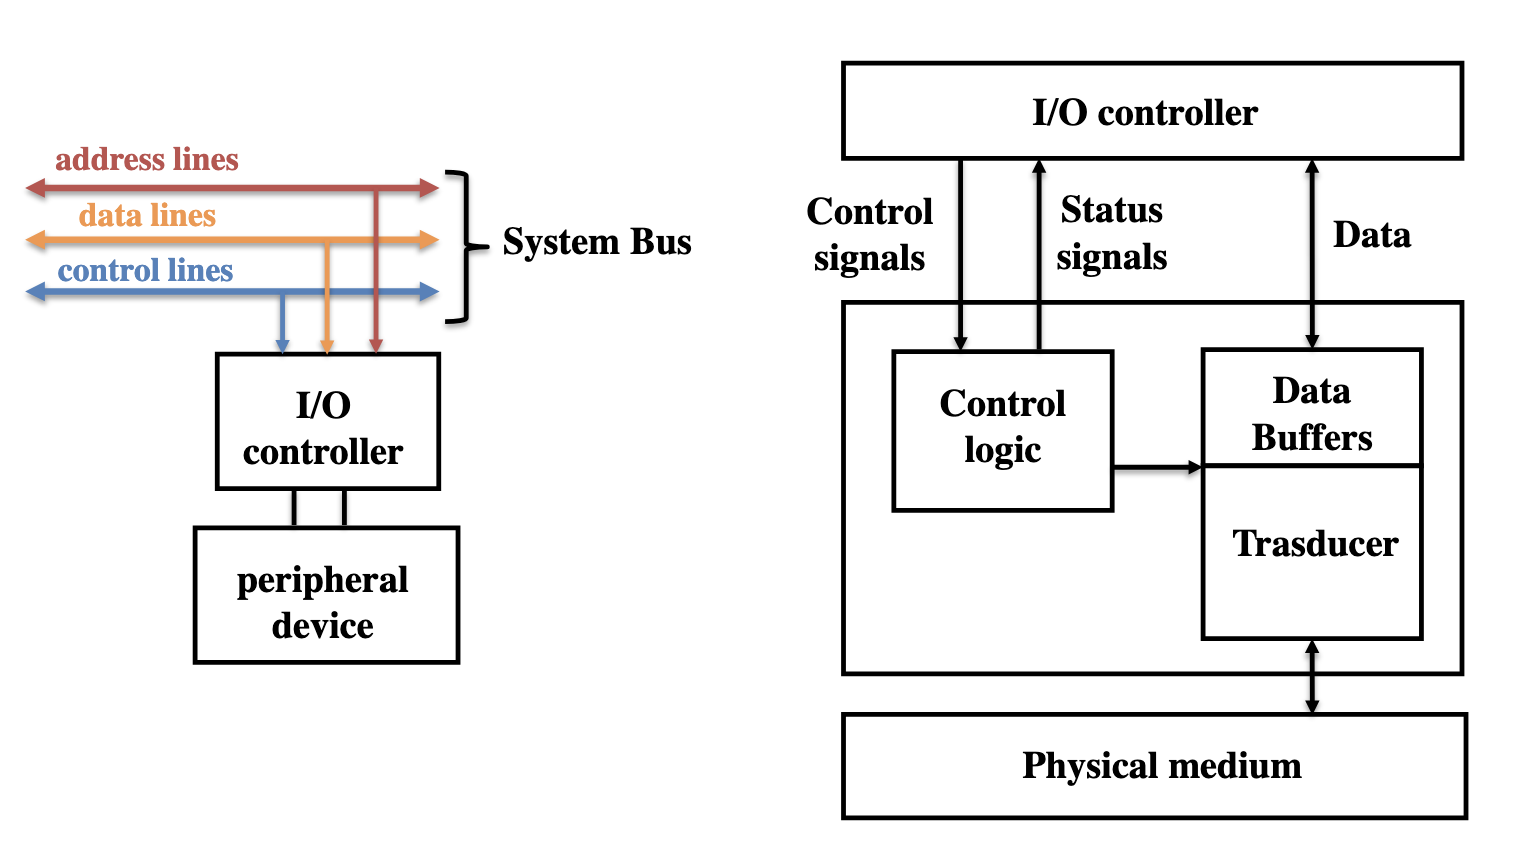
\includegraphics[width=12cm]{images/generic-io-device.png}
    \caption{I/O device generico}
\end{figure}

\hspace{-15pt}I/O funzioni di controllo abbiamo invece il control and imting, la comunicazioni fra processi (command decoding, data exchange, status reporting, address recognition), comunicazione
fra i device, il data buffering (per ottimizare il trasferimento dei dati e compensare le differenze di velocità).

\subsection{Connessione bus}
Servono per il controllo del trasferimento da un dispositivo al processore:
\begin{enumerate}
    \item la CPU controlla lo stato del dispositivo del modulo I/O.
    \item Il controller I/O restituisce lo stato se pronta.
    \item La CPU richiede il trasferimento dei dati tramite un comando al controllore.
    \item Il controller I/O riceve i dati dal dispositivo periferico.
    \item il controller I/O trasferisce i dati al processore.
\end{enumerate}

\begin{wrapfigure}{r}{7cm}
    \vspace{-35pt}
    \centering
    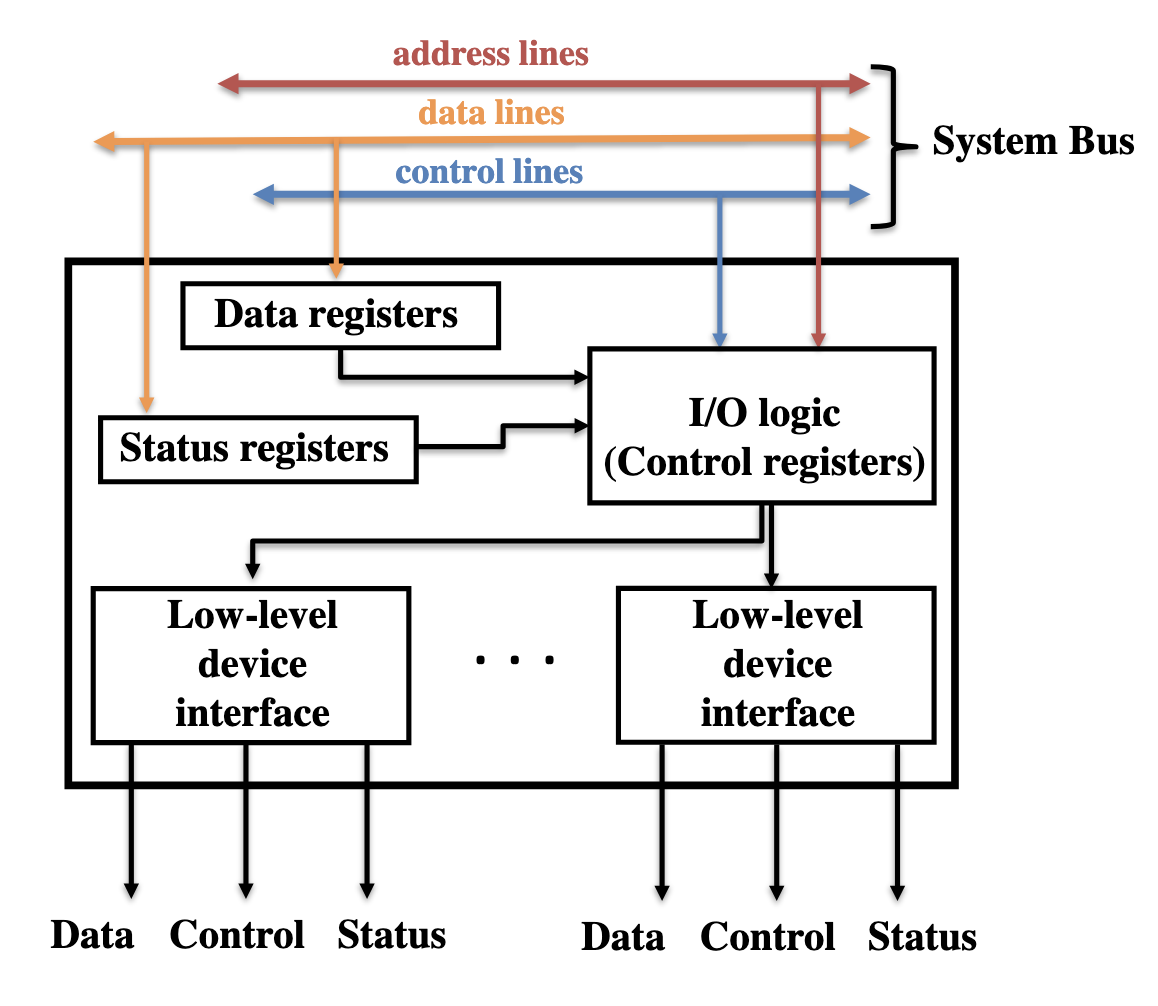
\includegraphics[width=6cm]{images/io-controller-diagram.png}
    \caption{I/O device generico}
\end{wrapfigure}
Questi passaggi richiedono una o più azioni di arbitrato del bus per implementare il protocollo di comunicazione.
Andiamo ora a definire l'interconnesione fra bus, essa si definisce come una raccolta di linee di dati trattate insieme come un singolo segnale logico
utilizzato anche per indicare una raccolta condivisa di linee con più dispositivi connessi (chiamati rubinetti), si definiscono su essi alcuni fattori di prestazione: lunghezza fisica, numero di prese collegate.
\\\\Un bus è un mezzo di trasmissione condiviso, solo un dispositivo alla volta può trasmettere con successo. Il bus di sistema collega i principali componenti (processore, memoria, bus I/O), centinaia di linee separate, linee classificate in tre gruppi: dati, indirizzo, controllo.
\newpage

% \begin{wrapfigure}{l}{2.5cm}
%     \centering
%     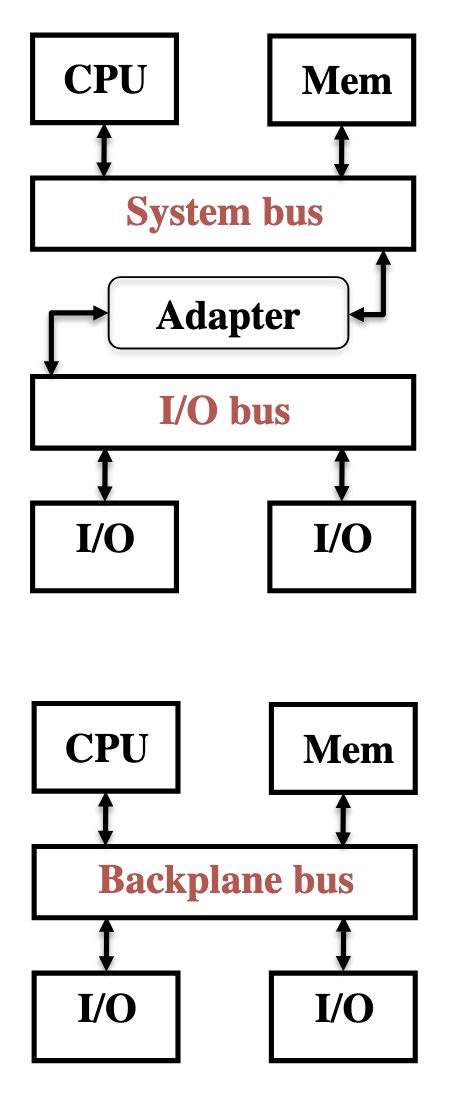
\includegraphics[width=2.5cm]{images/buses-type.png}
% \end{wrapfigure}
\hspace{-15pt}Alcuni tipi di bus sono:
\begin{itemize}
    \item \textbf{System bus} Collega processore e memoria, I/O interfacciato con adattatori: breve, pochi tocchi e quindi più veloce e larghezza di banda elevata, inoltre non è standard (ovvero specifico del sistema).
    \item \textbf{I/O bus} Connette dispositivi I/O, nessuna connessione diretta con processore e memoria: più tempo, più tocchi è uguale a più lentezza e larghezza di banda inferiore. E' uno standard di settore (ad es. ATA/SCSI).
    \item \textbf{Backplane bus} Connette CPU, memoria, dispositivi I/O. Lunghe, molti tocchi allora lento e larghezza di banda medio/bassa. Gestisce diversi dispositivi con diverse larghezze di banda ed è standard di settore.
\end{itemize}

\subsubsection{Bus design}
Il design di un bus si basa su soddisfare gli obbiettivi di avere un alta performance, standardizzazione e bassi costi. Per esempio 
il bus di sistema enfatizza le prestazioni, l'I/O e i bus backplain enfatizzano i costi e la standardizzazione.\\
Uno dei problemi principali di progettazioni da affrontare è il seguente: 
\begin{itemize}
    \item I cavi sono condivisi o separati? La risposta è che i bus più ampi (ovvero, una maggiore larghezza di banda) sono più costosi e più suscettibili allo skew.
    \item Come viene acquisito e rilasciato il controllo del bus? La riposta è tramite due metodologie \textbf{Atomic transactions} che permette una bassa utilizzazione ed una bassa complessita, e le \textbf{Split-transactions}
    dove le richieste/risposte possono essere intervallate; ciò significa un utilizzo più elevato ma un design più complesso (ad es. ID per identificare richieste diverse).
    \item Il bus ha è cloccato (ha un tempo di clock)? Per rispondere al problema del clock bisogna introdurre due opzioni possibili.
    \begin{itemize}
        \item \underline{\textbf{Sincrono}}. Tutti i dispositivi collegati al bus condividono lo stesso bus clock. Gli eventi si verificano all'estremità del segnale di clock. Un protocollo possibile è che al ciclo \(X\) l'unità di I/O scrive una richiesta READ sul bus; al ciclo \(X + \Delta\) l'unità può leggere i dati dal bus.
        \(\Delta\) è il tempo massimo per scrivere i dati sul bus da parte di un'unità collegata.\\
        Potenziale abbiamo il problema di skew dell'orologio e questa soluzione è limitata a bus brevi (ad esempio, bus di sistema).
        \item \underline{\textbf{Asincrono}}. Il bus non ha il clock. Nessun disallineamento dell'orologio, si occupa di dispositivi con velocità diverse: può essere più lungo, quindi più lento. \\
        Richiede protocolli di handshaking. Inoltre il protocollo possibilo funzione nel seguente modo (3 linee di controllo, 1 linea dati in cui i dati e l'indirizzo sono multiplexati): UIO1 scrive una richiesta READ (WRITE) ReadReq (WriteReq) nella linea di controllo e 
        l'indirizzo nella linea dati, UIO2 legge il indirizzo e scrive un ACK nella linea di controllo a UIO13. UIO2 scrive i dati sul bus e scrive la riga DataReadycontrol per notificare UIO14. UIO1 legge i dati e invia un ACK nella linea di controllo a UIO2.
    \end{itemize}
    \item Come si devide chi prende un bus per trasferire dati? Le comunicazioni bus devono essere gestite da un protocollo di comunicazione. Ne possiamo vedere due:
    \begin{itemize}
        \item \underline{\textbf{Bus master}}. Il concetto dietro questo protocolle è che, un unità che può avviare una richiesta di bus. Esso ha una configurazione più semplice: un solo master mentre di solito i bus hanno più master.
        \item \underline{\textbf{Arbitration}}. Il concetto invece di questo protocolle è che si va ha scegliere un master tra più richieste cercando di implementare la priorità e l'equità (prevenendo la fame). Solo un master alla volta (tutti gli altri ascoltano il bus). Il ruolo dell'arbitro è gestire le richieste del bus e assegnare le sovvenzioni considerando le priorità e l'equità.\\\\
        Per andare ad implementale questo sistema possiamo usare un metodo \textbf{centralizzato}, dove un dispositivo dedicato (Arbiter) raccoglie le richieste e poi decide (potenziale problema di collo di bottiglia). Si può usare un metodo ri raccolta Daisy-chain, non equo, oppure con linee di richiesta/risposta indipendenti (ampiamente utilizzate).
        \\\\Oppure possiamo usare un metodo \textbf{distribuito} dove ogni dispositivo vede le richieste contemporaneamente e partecipa alla selezione del master successivo (più complesso da realizzare e necessita di molte linee di controllo).
    \end{itemize}
\end{itemize}


\subsection{Gestione dell I/O}
Quando andiamo a parlare di gestione dei dispositivi di input output ci chiedimao come la CPU da i comandi 
hai dispositivi di I/O? Come la CPU sa quando i dispositivi di I/O completando le operazioni? Come fanno i 
disponsitivi di I/O ad eseguire il data transfers?\\\\
Partiamo dal rispondere alla prima domanda. Inanzitutto soltato il sistema operativo può mandare comandi hai dispositiv
di I/O ed i programmatori per mandare comandi all'I/O deve utilizzare delle chiamate di sistema. Da qui possiamo avere
due opzioni per mandare comandi hia device di I/O:
\begin{itemize}
    \item I/O istruzioni: istruzioni ISA che indirizzano i registri dei dispositivi I/O. Sono delle istruzioni di privilegio disponibile soltato in kernel mode.
    \item Memory-mapped I/O: una porzione degli indirizzi fisici rispervata all'I/O.
\end{itemize}

\hspace{-15pt}

\subsection{Memory-mapped I/O}
I registri interni dei dispositivi sono mappati su locazioni di memoria principali (a indirizzi fisici riservati). 
I comandi di I/O sono lettura/scrittura di memoria standard. Le operazioni in quelle posizioni vengono reindirizzate ai controller del dispositivo dalla MMU. 
Gli accessi in modalità utente alle aree mappate in memoria generano eccezioni di violazione della memoria.

\subsection{Programmed I/O}
Per andare invece ora a rispondere alla seconda domanda che era stata posta. Come la CPU sa quando i dispositivi di I/O completando le operazioni?
Introduciamo due concetti che possano risolvere questo probelma:
\begin{itemize}
    \item Programmed I/O: la cpu gestisce direttamente le operazioni e gli status di I/O.
    \item Interrupt-driven I/O: Un interrupt è un evento asincrono proveniente da un dispositivo (ad es. modulo I/O, timer, controller DMA). A volte le eccezioni sono anche c
    hiamate interruzioni (o comprendono interruzioni). In generale, le eccezioni sono eventi sincroni che interrompono l'esecuzione del programma (ad esempio, overflow aritmetico, istruzione non definita).
\end{itemize}

\hspace{-15pt}Nel caso specifico del programmed I/O come scritto sopra la CPU ha un diretto controllo sopra l'I/O, quindi 
gestisce lo stato di rilevamento, i comandi di lettura e scrittura ed il trasferimento dei dati. Con questo sistema i ll dispositivo I/O ha un ruolo passivo e 
la CPU attende che il modulo I/O completi le operazioni (polling). \\\\
Nel pulling il processore interroga il registro di stato del dispositivo I/O. Esso ha come pro una facile implmentazione
mentre come contro una perdita di cicli del processore perchè la CPU è molto più veloce che i dispositivi di I/O. La cpu deve leggere lo sato dei registri
molte volte solo per scoprire che il dispositivo non ha completato l'operazione.

\subsection{Interrupt-driven I/O}
Il problema principale visto nel programmed I/O è la perdita di tempo per l'alta velocità della CPU, come alternativa al polling
si introduce quello che viene chiamato interrupts.
\begin{itemize}
    \item La CPU invia comandi a un dispositivo e continua a svolgere altre attività. 
    \item Il dispositivo I/O genera un interrupt quando lo stato cambia, cioè i dati sono pronti.
    \item Gli interrupt di I/O sono asincroni.
    \item I/O interrupts sono prioritari, dove in particolare i dispositivi I/O con larghezza di banda elevata hanno una priorità maggiore rispetto a quelli con larghezza di banda ridotta.
\end{itemize} 

\hspace{-15pt}Dal punto di vista della CPU viene inviato un comando I/O (ad esempio, un carico mappato in memoria), nel fra tempo viene fatto altro lavoro, viene poi controllato l'interrupt alla fine del ciclo fetch-execute
e se l'iterrupt viene ricevuto salva il contesto corrente (ovvero i registri, non necessariamente tutti) e passa al livello privilegiato (ovvero PL1 su processore ARM), sulla base dell'ID dell'interrupt e della priorità dell'interrupt, il gestore dell'interrupt associato è pronto per essere eseguito, \footnote{I passaggi precedenti sono atomici dal punto di vista del sistema operativo!} 
esegui poi il gestore (ovvero, il sistema operativo gestisce l'interrupt) e ripristina il contesto per l'esecuzione dell'istruzione successiva: \footnote{il ripristino è un'operazione atomica per il sistema operativo! }

\begin{example}
    Facciamo ora un esempio, assumiamo di avere una CPU ad una velocità di 500MHz ed un costo di polling di 400 cicli. Abbiamo poi un mouse come dispositivo a banda lenta.
    Vogliamo aver un poll di 30 volte al secondo.\\\\
    Per calcolare i cicli al secondo per polling scriviamo (30 poll/s) * 400 = 120000 cycles/s, e la percentuale di cicli spesi
    per polling si calocla fancendo 12K/500M = 0.002\(\%\). Abbiamo dunque un overhead accettabile.\\\\
    Prendiamo ora un disco (che è un dispositivo ad alta lunghezza si banda) che ha 4MB/s di transfer rate e 16B interface.\\
    Per non mancare i dati dobbiamo eseguire il poll abbastanza spesso, quindi (4MB/s)/16B = 250 K/s, vista come percentuale di cicli
    abbiamo 100M / 500 M = 20\(\%\), questo risultato non è accetabile perchè Abbiamo speso il 20\(\%\) dei cicli solo per controllare i registri I/O, non per il trasferimento dei dati
\end{example}

\subsection{Data transfers (DMA)}
Andiamo ora a rispondere all'ultima domanda che ci eravamo posti, come i device di I/O eseguno il trasferimento dei dati?
Sappiamo ora che l'I/O guidato da interrupt elimina i problemi di polling, tuttavia, il sistema operativo deve trasferire i dati una parola alla volta. Questo va bene solo per dispositivi I/O a bassa larghezza di banda (ad es. mouse), per ovviare
a questo problma introduciamo la direct memory access (DMA).\\\\
Esso è meccanismi che forniscono a un dispositivo di controllo I/O la capacità di trasferire i dati direttamente da e verso la memoria principale senza coinvolgere la CPU. 
DMA disaccoppia il protocollo CPU-memoria dal protocollo memoria-dispositivo I/O. Interrupt utilizzati dal dispositivo I/O per comunicare con la CPU solo al completamento del trasferimento I/O o quando si verifica un errore.\\\\
DMA è implementato con un controller specializzato. Per eseguire DMA, un dispositivo I/O è collegato a un controller DMA: è possibile collegare più dispositivi allo stesso controller. Il controller stesso è visto come un dispositivo I/O mappato in memoria, 
inoltre il controller DMA si occupa dell'arbitrato del bus e del trasferimento dei dati: diventa il master del bus. Il controller DMA e la CPU si contendono il bus di memoria.
Ci sono tre passi nel transfer DMA:
\begin{enumerate}
    \item La CPU imposta DMA fornendo identità, op, indirizzo di memoria e numero di byte da trasferire.
    \item DMA avvia l'operazione sul dispositivo e arbitra la connessione. Trasferisce i dati dal dispositivo o dalla memoria.
    \item Una volta completato il trasferimento DMA, il controller invia un interrupt alla CPU.
\end{enumerate}

\begin{example}
    Facciamo un esempio, assumiamo i seguenti dati: 500Mhz CPU, il device di un disco ha un tempo di trasferimento 4MB/s, 16B di interfaccie
    e un utilizzo di 50\(\%\), la gestione degli interrupt richiede 400 cicli, il trasferimento dei dati richiede 100 cicli, l'installazione DMA richiede 1600 cicli, trasferisce un blocco da 16 KB alla volta.\\\\
    Overhead del processore per I/O guidato da interrupt senza DMA (il processore è coinvolto per ogni trasferimento di dati (16 B)) si calcola facendo 0.5 * (4MB/s) / (16B) * [(400 + 100) cicli / 500M cicli/s] = 12.5 \(\%\).\\\\
    Overhead del processore per I/O guidato da interrupt con trasferimento DMA (Il processore è coinvolto una volta per trasferimento a blocchi (16 KB)) si calcola invece facendo 0.5 * (4M B/s) / (16KB) * [(1600 + 400) / (5ooM cicli/s)] = 0.05 \(\%\)
\end{example}

\hspace{-15pt}Notiamo da questo esempio che Senza DMA: il processore avvia tutti i trasferimenti di dati, tutti i trasferimenti passano attraverso la traduzione degli indirizzi (MMU), i trasferimenti possono essere di qualsiasi dimensione e attraversare i limiti della pagina virtuale, 
nessun impatto sulla gerarchia della cache, le cache non contengono mai dati obsoleti.\\\\
Mentre con DMA: il controller DMA avvia i trasferimenti di dati, esiste un altro percorso per il sistema di memoria, potenziali problemi: 
i controller DMA utilizzano indirizzi virtuali o fisici? Cosa succede se scrivono i dati in una posizione di memoria cache?\\\\
Per rispondere alla domanda, quali indirizzi il processore specifica al controller DMA? Abbiamo la virtual DMA e la 
DMA fisica:
\begin{itemize}
    \item Virtual DMA: Il controller DMA deve eseguire internamente la traduzione degli indirizzi utilizzando una piccola cache (TLB) inizializzata dal sistema operativo quando richiede un trasferimento I/O. Complesso ma flessibile (ad esempio, grandi trasferimenti tra pagine).
    \item Physical DMA: Il controller DMA funziona con indirizzi fisici. Trasferimenti alla granularità della pagina, il sistema operativo suddivide i trasferimenti di grandi dimensioni in blocchi delle dimensioni della pagina. Più semplice, ma meno flessibile.
\end{itemize}

\hspace{-15pt}La DMA ha anche un'integrazione con la cache essendo che la memorizzazione nella cache riduce le istruzioni della CPU e la latenza di accesso ai dati e riduce l'utilizzo della memoria da parte della CPU, lasciando così più larghezza di banda di memoria/bus per i trasferimenti DMA. Ma le cache introducono un problema di coerenza per DMA: se il DMA scrive nella memoria principale, la versione dei dati nella cache è obsoleta. Per le cache write-back, il controller DMA potrebbe leggere i vecchi valori dei dati dalla memoria mentre i dati nella cache hanno il set di bit sporchi. La soluzione è lo svuotamento/invalidamento selettivo delle linee memorizzate nella cache 
coinvolte nei trasferimenti DMA: richiede una logica aggiuntiva per la coerenza della cache HW!\\\\
L'accesso hai device è gestito tramite, uno stack software che fornisce modi per accedere a un'ampia gamma di dispositivi I/O. 
Un'interfaccia comune, in POSIX equivalente all'accesso ai file, in termini di chiamate di sistema 
di apertura/chiusura, lettura/scrittura. Driver di dispositivo per ogni dispositivo specifico, parte superiore HW, 
indipendenti (per migliorare la portabilità), parte inferiore HW-dipendente


